% Options for packages loaded elsewhere
\PassOptionsToPackage{unicode}{hyperref}
\PassOptionsToPackage{hyphens}{url}
%
\documentclass[
]{article}
\usepackage{lmodern}
\usepackage{amssymb,amsmath}
\usepackage{ifxetex,ifluatex}
\ifnum 0\ifxetex 1\fi\ifluatex 1\fi=0 % if pdftex
  \usepackage[T1]{fontenc}
  \usepackage[utf8]{inputenc}
  \usepackage{textcomp} % provide euro and other symbols
\else % if luatex or xetex
  \usepackage{unicode-math}
  \defaultfontfeatures{Scale=MatchLowercase}
  \defaultfontfeatures[\rmfamily]{Ligatures=TeX,Scale=1}
\fi
% Use upquote if available, for straight quotes in verbatim environments
\IfFileExists{upquote.sty}{\usepackage{upquote}}{}
\IfFileExists{microtype.sty}{% use microtype if available
  \usepackage[]{microtype}
  \UseMicrotypeSet[protrusion]{basicmath} % disable protrusion for tt fonts
}{}
\makeatletter
\@ifundefined{KOMAClassName}{% if non-KOMA class
  \IfFileExists{parskip.sty}{%
    \usepackage{parskip}
  }{% else
    \setlength{\parindent}{0pt}
    \setlength{\parskip}{6pt plus 2pt minus 1pt}}
}{% if KOMA class
  \KOMAoptions{parskip=half}}
\makeatother
\usepackage{xcolor}
\IfFileExists{xurl.sty}{\usepackage{xurl}}{} % add URL line breaks if available
\IfFileExists{bookmark.sty}{\usepackage{bookmark}}{\usepackage{hyperref}}
\hypersetup{
  pdftitle={Supplementary material, Geographical imprints of trait evolution in evolutionary radiations},
  pdfauthor={André Luza},
  hidelinks,
  pdfcreator={LaTeX via pandoc}}
\urlstyle{same} % disable monospaced font for URLs
\usepackage[margin=1in]{geometry}
\usepackage{graphicx,grffile}
\makeatletter
\def\maxwidth{\ifdim\Gin@nat@width>\linewidth\linewidth\else\Gin@nat@width\fi}
\def\maxheight{\ifdim\Gin@nat@height>\textheight\textheight\else\Gin@nat@height\fi}
\makeatother
% Scale images if necessary, so that they will not overflow the page
% margins by default, and it is still possible to overwrite the defaults
% using explicit options in \includegraphics[width, height, ...]{}
\setkeys{Gin}{width=\maxwidth,height=\maxheight,keepaspectratio}
% Set default figure placement to htbp
\makeatletter
\def\fps@figure{htbp}
\makeatother
\setlength{\emergencystretch}{3em} % prevent overfull lines
\providecommand{\tightlist}{%
  \setlength{\itemsep}{0pt}\setlength{\parskip}{0pt}}
\setcounter{secnumdepth}{-\maxdimen} % remove section numbering

\title{Supplementary material, Geographical imprints of trait evolution in
evolutionary radiations}
\author{André Luza}
\date{31/08/2021}

\begin{document}
\maketitle

\hypertarget{appendix-s2-results-considering-the-set-of-100-fully-resolved-phylogenies-but-considering-the-216-species-that-had-occurrence-traits-and-phylogenetic-data-and-the-species-belonging-to-the-clade-oryzomyialia.}{%
\subsubsection{Appendix S2: Results considering the set of 100 fully
resolved phylogenies, but considering the 216 species that had
occurrence, traits and phylogenetic data, and the species belonging to
the clade
Oryzomyialia.}\label{appendix-s2-results-considering-the-set-of-100-fully-resolved-phylogenies-but-considering-the-216-species-that-had-occurrence-traits-and-phylogenetic-data-and-the-species-belonging-to-the-clade-oryzomyialia.}}

This is a document that reports alternative results of our paper. Here
we show figures similar to the ones showed in the main text. The first
one is the relationship between SES MPD (mean pairwise (phylogenetic)
distance between species) and SES disparity regarding the empirical
skull dataset, and three datasets generated by trait simulation
(Brownian motion, Early-Burst, and OU). The second one is a panel with
maps of empirical and SES disparity found for each evolutionary model,
as well correlation between these estimates.

\hypertarget{species}{%
\paragraph{216 species}\label{species}}

The first thing we did was to show the bivariate plot describind the
relationship between SES disparity and SES MPD, for empirical and
simulated datasets, also was similar to the one reported in the main
results (Fig. 2 in the main text). Overall, the disparity produced by
the EB model had a closer relationship with the empirical disparity than
other models of evolution (OU and BM). However, phylogenetic uncertainty
(as shown by the boxplots) was much higher here --mainly for EB -- than
when using the phylogeny with 413 species to simulate the trait.

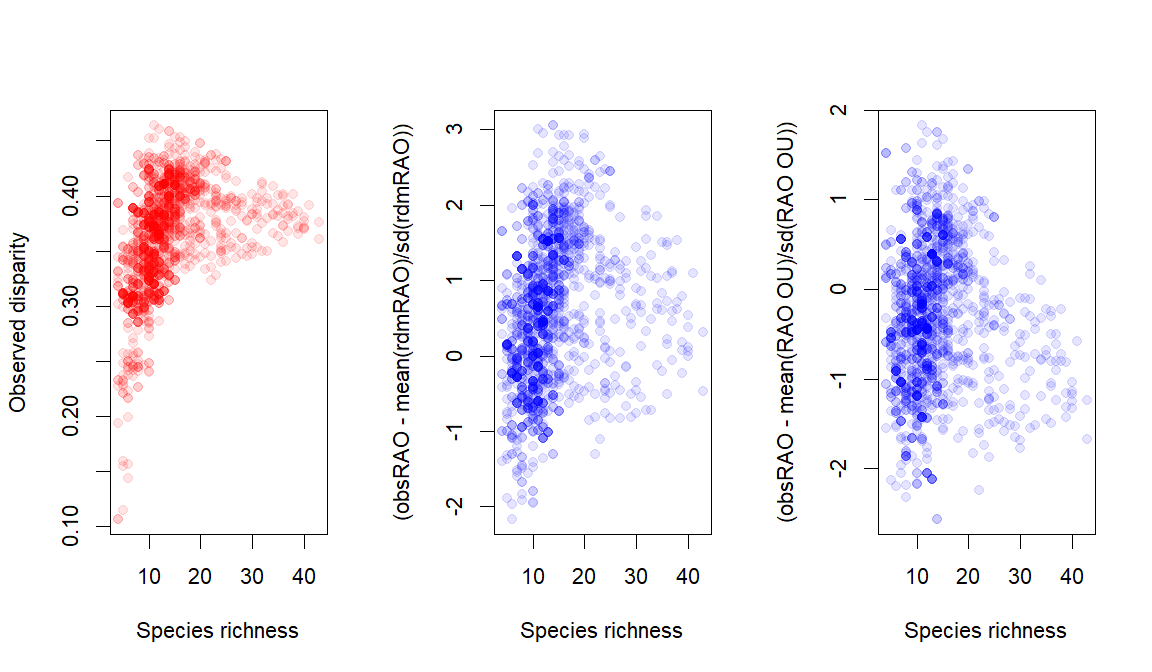
\includegraphics{index_files/figure-latex/unnamed-chunk-1-1.pdf}

Then we counted the number of cells in the map with values of disparity
higher, equal, or lower than the null model (including randomization,
NULL) and evolutionary models (OU, BM, EB). As can be seen, the number
of cells with values of disparity higher, equal, or lower than the null
model and evolutionary models was pretty similar to the number reported
in the main results.

\begin{verbatim}
## $lower
##      lowerNULL lowerOU lowerBM lowerEB
## TRUE       509     258     134       8
## 
## $higher
##      highNULL highOU highBM highEB
## <NA>       NA      7     12    141
\end{verbatim}

When mapping the values of empirical and simulated trait values, we
found a high agreement between the following maps and the ones showed in
Fig. 3 of main text. The null disparity, as produced by a null model of
random shuffling of species labels (rows) in the trait table, produces
underestimated values of disparity (as shown in B, blue color). In
contrast, the estimates of a BM model produced {[}smoother{]} estimates
(C).

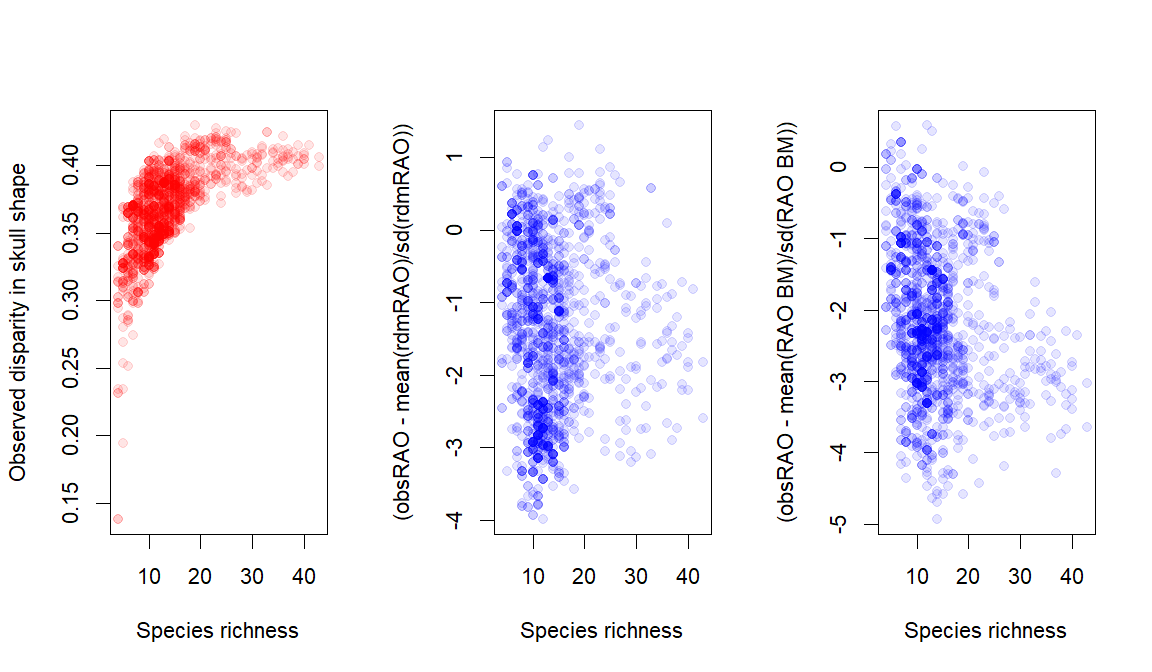
\includegraphics{index_files/figure-latex/unnamed-chunk-2-1.pdf}

We also show that using a null model is quite similar than simulation a
trait using the OU model. This can be seen in the following map, where
the null disparity and the disparity produced by the OU model produced
quite similar maps, and estimates were highly correlated (0.98, Table
below the map). The correlation also was high between the Null and BM
disparity.

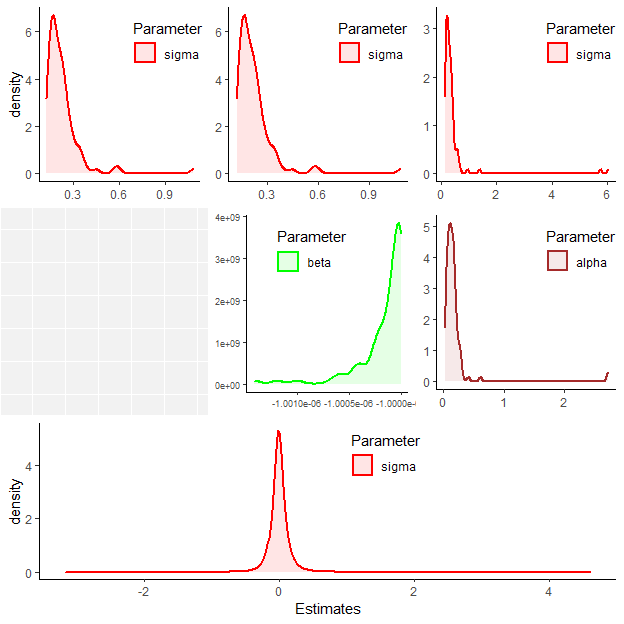
\includegraphics{index_files/figure-latex/unnamed-chunk-3-1.pdf}

Table of correlation between these estimates

\begin{verbatim}
##                  RAO_OBS.med_nulo     obsBM     obsEB     obsOU
## RAO_OBS.med_nulo        1.0000000 0.9354015 0.5486150 0.9832293
## obsBM                   0.9354015 1.0000000 0.7663491 0.8952412
## obsEB                   0.5486150 0.7663491 1.0000000 0.4669195
## obsOU                   0.9832293 0.8952412 0.4669195 1.0000000
\end{verbatim}

Finally the map of significance of SES disparity to show which places
have a disparity that deviates -1.96 or +1.96 standard deviations from
zero. What we see in this map is that: 1) the null model often
underestimate disparity, now shown by the significance of the SES
disparity, resulting in SES disparity lower than the null expectation at
most of the Neotropics; 2) Atlantic Rainforest has communities with much
higher disparity than expected by the evolutionary models.

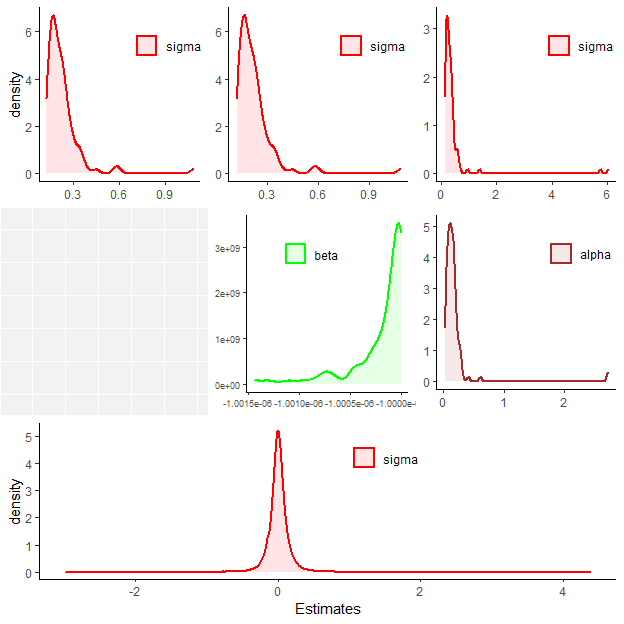
\includegraphics{index_files/figure-latex/unnamed-chunk-5-1.pdf}

\hypertarget{oryzomyialia}{%
\paragraph{Oryzomyialia}\label{oryzomyialia}}

Bivariate plot similar to Fig. 2. This is pretty similar to the results
in the main text and alternative results considering 216 species (just
presented). However, the main difference is that we lost values of SES
MPD higher than zero, as now we're working only with closely related
species.

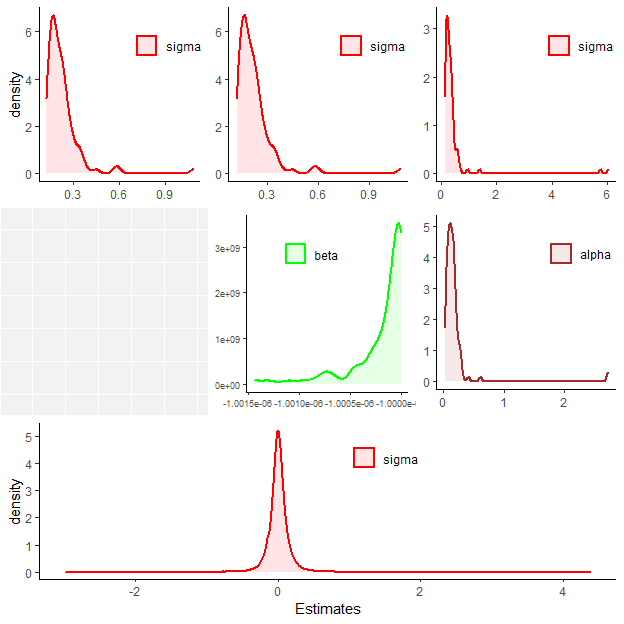
\includegraphics{index_files/figure-latex/unnamed-chunk-6-1.pdf}

Counting the number of cells. This is quite similar to the number
reported in the main text and results considering 216 species. The main
difference is that now we have some communities with disparity HIGHER
than the null disparity and BM-resulting disparity.

\begin{verbatim}
## $lower
##      lowerNULL lowerOU lowerBM lowerEB
## TRUE       384      77      54      17
## 
## $higher
##      highNULL highOU highBM highEB
## TRUE        1      1     NA     NA
\end{verbatim}

Map similar to Fig. 3, and map just reported considering 216 species.

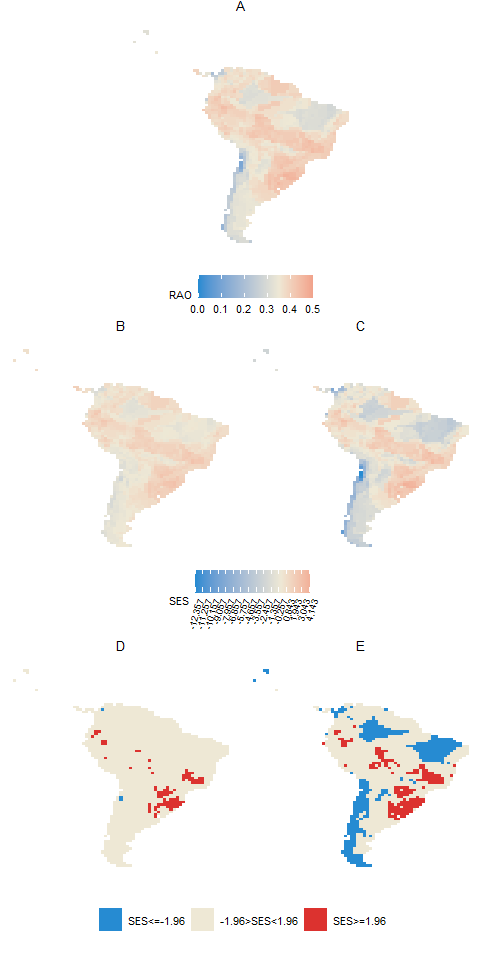
\includegraphics{index_files/figure-latex/unnamed-chunk-8-1.pdf}

Map similar to Fig. 4,

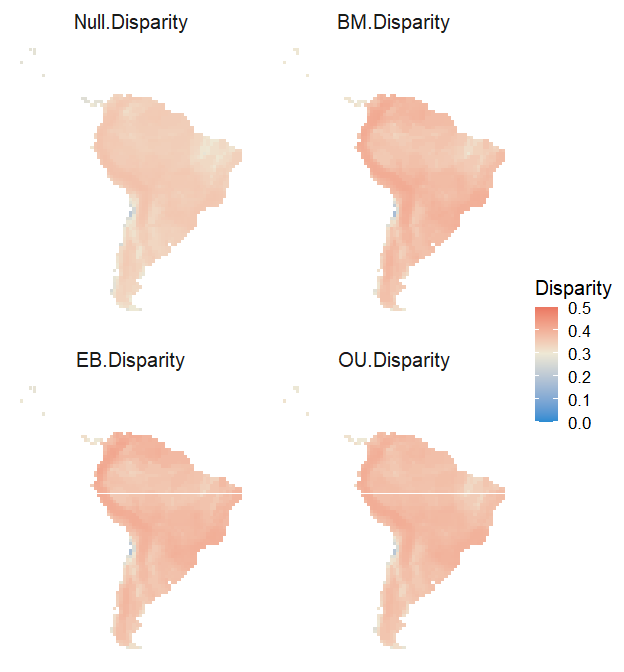
\includegraphics{index_files/figure-latex/unnamed-chunk-9-1.pdf}

as well correlations.

\begin{verbatim}
##                  RAO_OBS.med_nulo     obsBM     obsEB     obsOU
## RAO_OBS.med_nulo        1.0000000 0.9395127 0.7312169 0.9894764
## obsBM                   0.9395127 1.0000000 0.8999812 0.9496548
## obsEB                   0.7312169 0.8999812 1.0000000 0.7619259
## obsOU                   0.9894764 0.9496548 0.7619259 1.0000000
\end{verbatim}

At the end we show the map of significance of SES disparity for each
model. Now we don't have SES disparity higher than the expectations for
the many models along the Atlantic Rainforest.

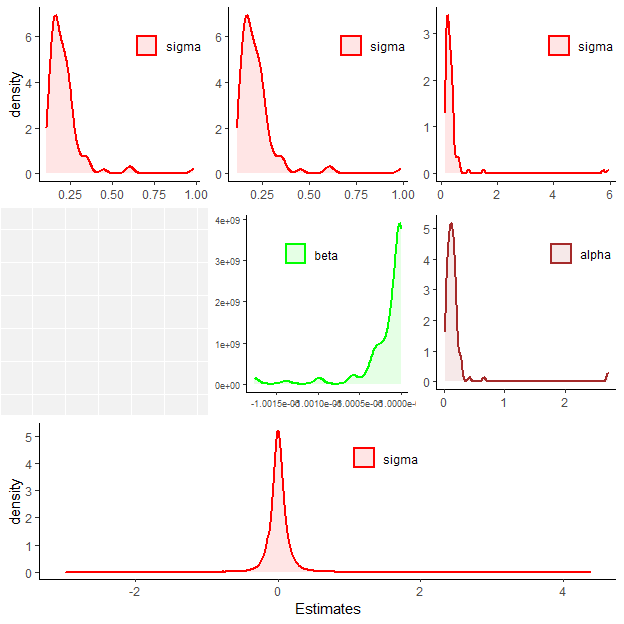
\includegraphics{index_files/figure-latex/unnamed-chunk-11-1.pdf}

\hypertarget{appendix-s3-results-considering-the-consensus-phylogeny.-as-it-has-285-tips-the-number-of-species-used-in-trait-simulation-was-285-169-all-species-with-occurrence-trait-and-phylogenetic-data-and-159-species-belonging-to-the-clade-oryzomyialia.}{%
\subsubsection{Appendix S3: Results considering the consensus phylogeny.
As it has 285 tips, the number of species used in trait simulation was
285, 169 (all species with occurrence, trait and phylogenetic data) and
159 species (belonging to the clade
Oryzomyialia).}\label{appendix-s3-results-considering-the-consensus-phylogeny.-as-it-has-285-tips-the-number-of-species-used-in-trait-simulation-was-285-169-all-species-with-occurrence-trait-and-phylogenetic-data-and-159-species-belonging-to-the-clade-oryzomyialia.}}

The figures have the same settings and order as the ones just presented.
Let's see \ldots{}

Bivariate plot similar to Fig. 2. The EB-resulting disparity is still
closer to the empirical disparity than other models.

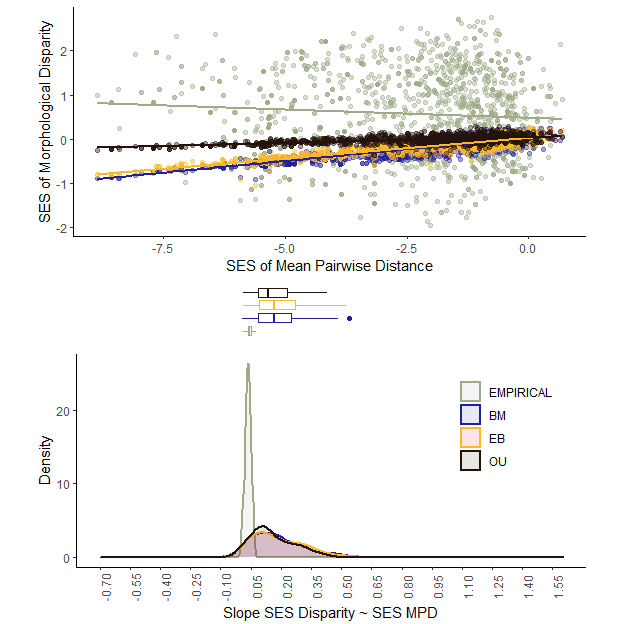
\includegraphics{index_files/figure-latex/unnamed-chunk-12-1.pdf}

Counting the number of cells. This is quite similar to the number
reported in the main text and results considering 216 species. The main
difference is that now we have some communities with disparity HIGHER
than the null disparity and BM-resulting disparity.

\begin{verbatim}
## $lower
##      lowerNULL lowerOU lowerBM lowerEB
## TRUE       460     257      NA      NA
## 
## $higher
##      highNULL highOU highBM highEB
## <NA>       NA     NA     NA     NA
\end{verbatim}

Map similar to Fig. 3, and map just reported considering 216 species.
The main difference is that the values of SES disparity are
\textasciitilde0.3 units higher (for positive and negative sides) than
the previous results we reported.

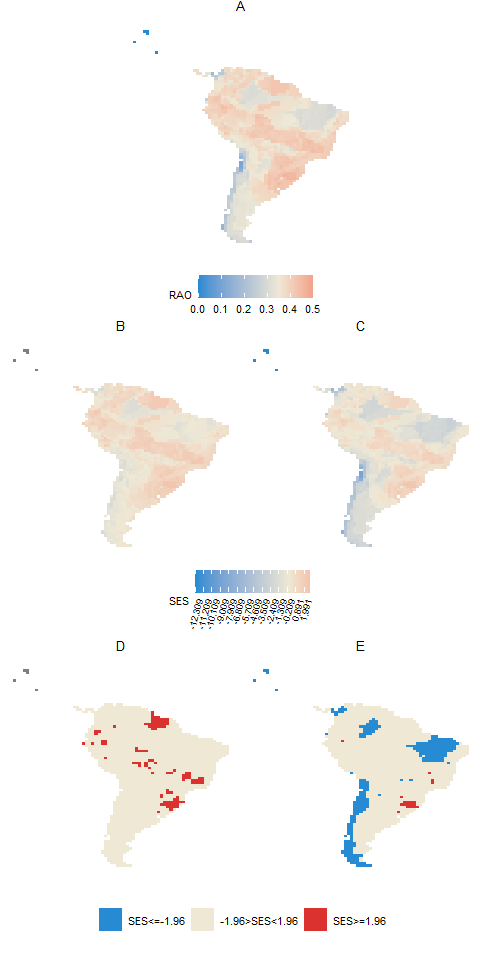
\includegraphics{index_files/figure-latex/unnamed-chunk-14-1.pdf}

Map similar to Fig. 4, but that now show little correlation between null
and evolution-based disparity.

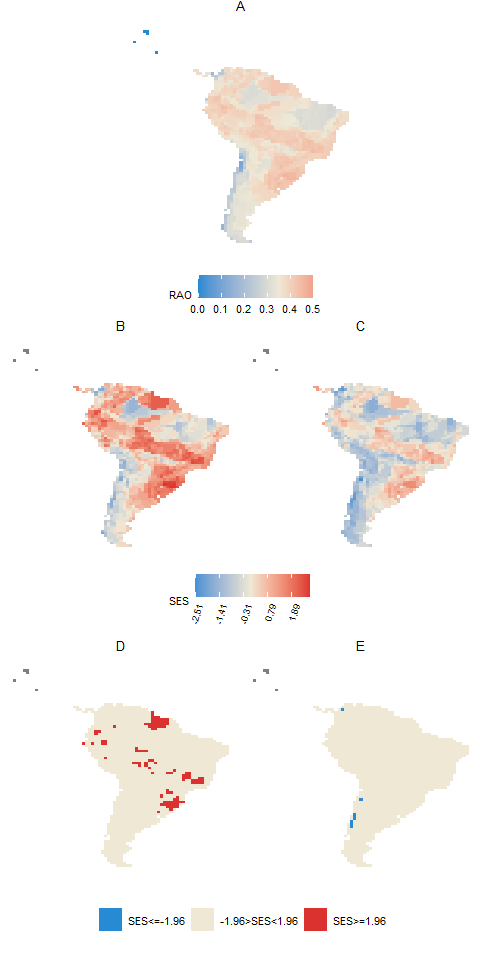
\includegraphics{index_files/figure-latex/unnamed-chunk-15-1.pdf}

and correlations are much lower than the ones reported in the previous
results and main text.

\begin{verbatim}
##                  RAO_OBS.med_nulo      obsBM     obsEB      obsOU
## RAO_OBS.med_nulo        1.0000000 0.23442243 0.2796173 0.19213008
## obsBM                   0.2344224 1.00000000 0.1578276 0.06870823
## obsEB                   0.2796173 0.15782758 1.0000000 0.37894289
## obsOU                   0.1921301 0.06870823 0.3789429 1.00000000
\end{verbatim}

At the end we show the map of significance of SES disparity for each
model. Now we don't have SES disparity higher or lower than expected by
EB and BM. Again the null model and OU seems to underestimated
disparity.

\includegraphics{index_files/figure-latex/unnamed-chunk-17-1.pdf}

These results mostly repeat considering 169 species with occurrence,
trait and phylogenetic data:

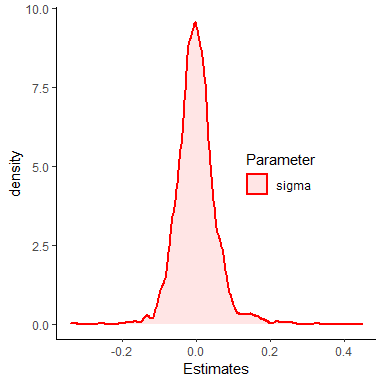
\includegraphics{index_files/figure-latex/unnamed-chunk-18-1.pdf}

Counting the number of cells.

\begin{verbatim}
## $lower
##      lowerNULL lowerOU lowerBM lowerEB
## TRUE       457      11      25      23
## 
## $higher
##      highNULL highOU highBM highEB
## <NA>       NA     NA     NA     NA
\end{verbatim}

Map similar to Fig. 3.

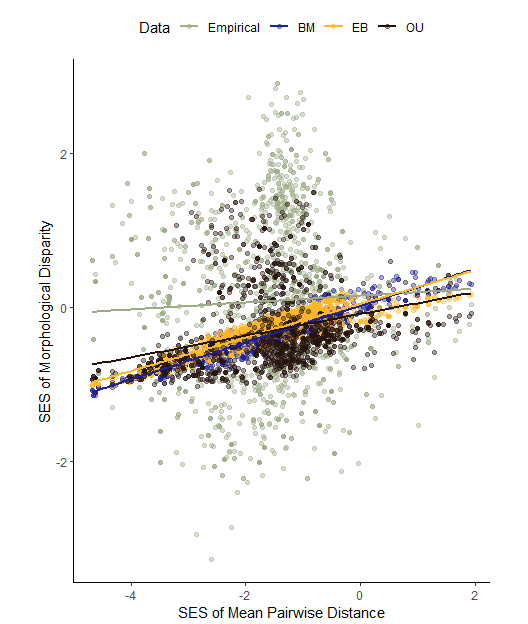
\includegraphics{index_files/figure-latex/unnamed-chunk-20-1.pdf}

Map similar to Fig. 4.

\includegraphics{index_files/figure-latex/unnamed-chunk-21-1.pdf}

and correlations.

\begin{verbatim}
##                  RAO_OBS.med_nulo     obsBM     obsEB     obsOU
## RAO_OBS.med_nulo        1.0000000 0.5560391 0.3829528 0.5204967
## obsBM                   0.5560391 1.0000000 0.3964583 0.3542735
## obsEB                   0.3829528 0.3964583 1.0000000 0.3037524
## obsOU                   0.5204967 0.3542735 0.3037524 1.0000000
\end{verbatim}

At the end we show the map of significance of SES disparity for each
model.

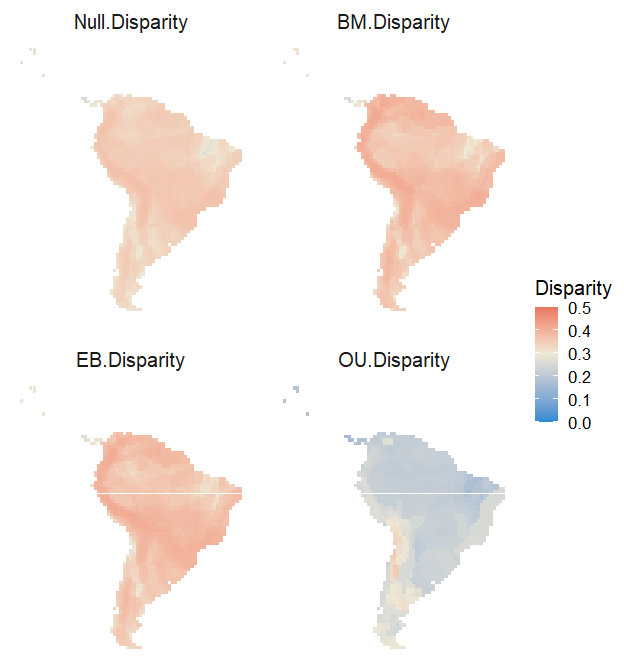
\includegraphics{index_files/figure-latex/unnamed-chunk-23-1.pdf}

And similar to Oryzomyialia as well.

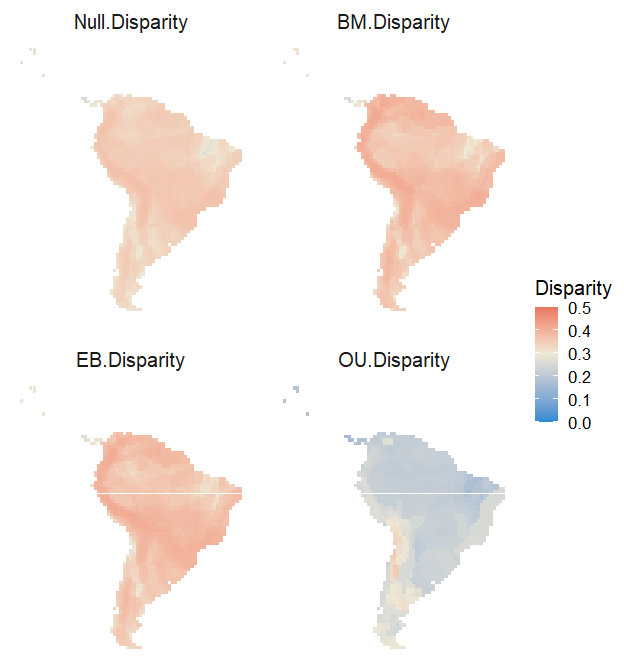
\includegraphics{index_files/figure-latex/unnamed-chunk-24-1.pdf}

Counting the number of cells.

\begin{verbatim}
## $lower
##      lowerNULL lowerOU lowerBM lowerEB
## TRUE       335      11       8      47
## 
## $higher
##      highNULL highOU highBM highEB
## TRUE        1     NA    100     NA
\end{verbatim}

Map similar to Fig. 3.

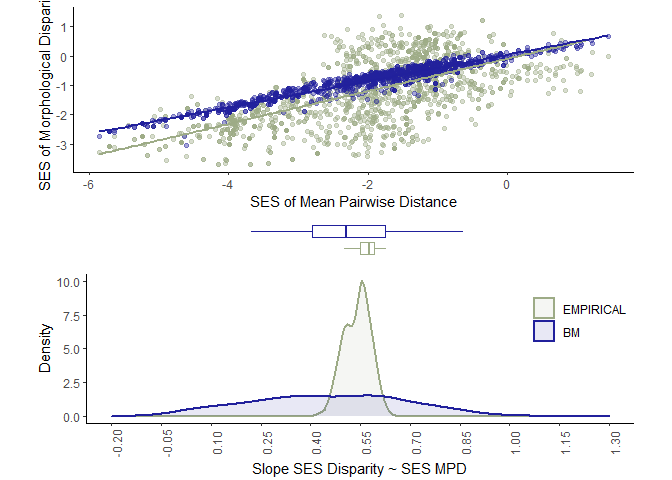
\includegraphics{index_files/figure-latex/unnamed-chunk-26-1.pdf}

\begin{verbatim}
## TableGrob (9 x 7) "arrange": 3 grobs
##   z     cells    name           grob
## 1 1 (1-5,2-6) arrange gtable[layout]
## 2 2 (6-9,1-4) arrange gtable[layout]
## 3 3 (6-9,5-7) arrange gtable[layout]
\end{verbatim}

Map similar to Fig. 4.

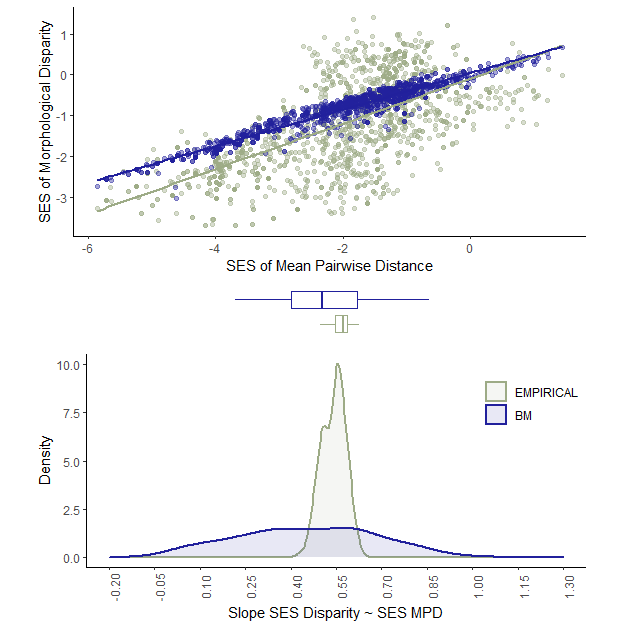
\includegraphics{index_files/figure-latex/unnamed-chunk-27-1.pdf}

and correlations.

\begin{verbatim}
##                  RAO_OBS.med_nulo     obsBM     obsEB     obsOU
## RAO_OBS.med_nulo        1.0000000 0.5531678 0.5553153 0.5128892
## obsBM                   0.5531678 1.0000000 0.2831670 0.2400483
## obsEB                   0.5553153 0.2831670 1.0000000 0.5826006
## obsOU                   0.5128892 0.2400483 0.5826006 1.0000000
\end{verbatim}

At the end we show the map of significance of SES disparity for each
model. This results supports the one reported in the main text
(divergent evolution in the Atlantic Rainforest)

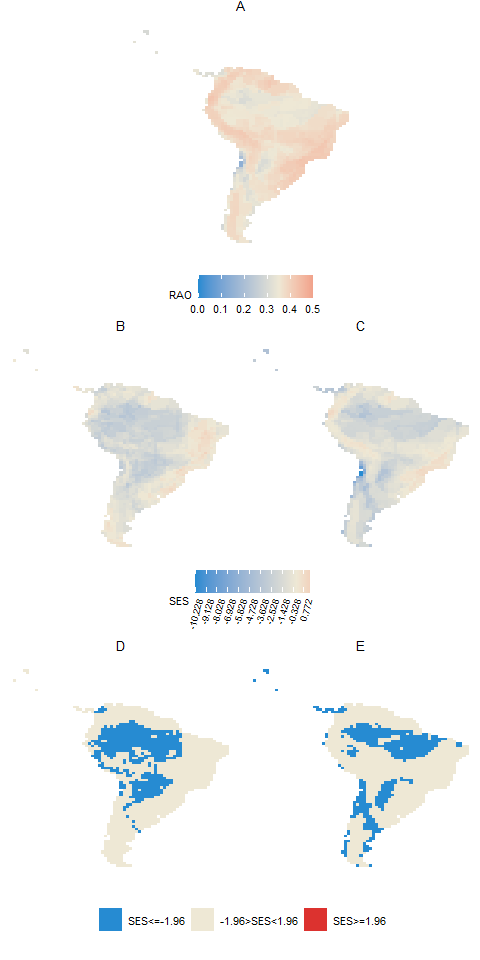
\includegraphics{index_files/figure-latex/unnamed-chunk-29-1.pdf}

\hypertarget{appendix-s4-sensitivity-of-results-to-model-parameters}{%
\subsubsection{Appendix S4: Sensitivity of results to model
parameters}\label{appendix-s4-sensitivity-of-results-to-model-parameters}}

Finally, we report results regarding different values of model
parameters.

To understand whether results were sensitive to model parameter values
(basically sigma for BM, sigma and beta for EB, and sigma and alpha for
OU), we ran sensitivity analyses in terms of how the regression
coefficient of SES disparity relative to SES MPD (SES disparity
\textasciitilde{} SES MPD) would change with data simulated using
different model parameters. We then simulated trait data using the
following values: \emph{sigma: 0.5, 1.0, 1.5, 2.0 (weak to strong rate
of random fluctuations) beta: -0.5, 0.0, 0.5, 1.0 (early to late burst)
alpha: 1.0 1.5 2.0 2.5 (weak to strong attraction to an average trait
value)}

Results presented in the main text show the similarity of the SES
disparity \textasciitilde SES MPD relationship regarding the empirical
and simulated disparity (BM-, EB- and OU-simulated disparity) (Fig. 2 in
the main). Here, we did the same analysis but now considering this range
of values of sigma, beta, and alpha. Remember that in the main text we
used: sigma = 1, beta = -0.5, and alpha = 1. Here we used the consensus
phylogeny to save processing time.

We found that the shape of the empirical SES disparity
\textasciitilde SES MPD relationship was quite similar to simulated SES
disparity \textasciitilde{} SES MPD across the alternative values of
sigma (Fig. S3.1). The slopes of simulated SES disparity
\textasciitilde{} SES MPD were less steeper than the slope produced by
empirical SES disparity \textasciitilde{} SES MPD, as reported in the
main results.

We found that the shape of the empirical SES disparity
\textasciitilde SES MPD relationship was quite similar to the simulated
SES disparity \textasciitilde{} SES MPD across the alternative values of
beta (Fig. S3.2) -- except to a late-burst model with beta = 1. SES
disparity calculated using traits simulated with values of beta = -0.5
and 0 produced a slope relative to SES MPD very closer to the slope
found for the empirical SES disparity.

Different values of alpha produced very different simulated SES
disparity relative to SES MPD -- since positive to neutral and negative
slopes (Fig. S3.3). Disregarding the alpha value, all relationships
produced slopes that were quite different relative to the slope of
empirical SES disparity \textasciitilde{} SES MPD reported in the main
text. Finally, neither BM nor OU (and alternative values of sigma and
alpha) produced a simulated SES disparity \textasciitilde{} SES MPD as
closer to the empirical SES disparity \textasciitilde{} SES MPD as the
EB model (as found in the main results).

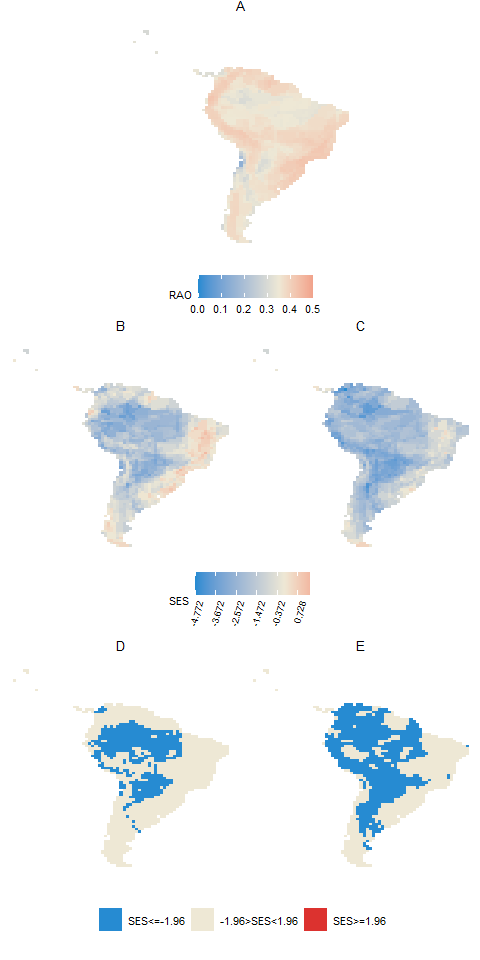
\includegraphics{index_files/figure-latex/unnamed-chunk-30-1.pdf}

\begin{verbatim}
## TableGrob (3 x 1) "arrange": 3 grobs
##   z     cells    name           grob
## 1 1 (1-1,1-1) arrange gtable[layout]
## 2 2 (2-2,1-1) arrange gtable[layout]
## 3 3 (3-3,1-1) arrange gtable[layout]
\end{verbatim}

Scatter plot showing the relationship between SES disparity and SES MPD
across different values of alpha (the parameter of OU evolution model).
The OU model also has a sigma parameter, and it was set to 1.

\end{document}
